\subsection{Git}
\subsubsection{Logiciel}
Git est un logiciel de gestion de code source et de version. Git capture l'état dans lequel se trouvent les fichiers à chaque nouvelle version. Il garde un historique de chaque version ajoutée afin de pouvoir facilement revenir en arrière, les comparer ou bien travailler sur une nouvelle version (branche) sans modifier celles existante. De plus, en partageant un dépôt commun, Git permet à plusieurs personne de travailler sur le même projet en résolvant quasi automatiquement les éventuels conflits (ou, à défaut, obliger les développeurs à les résoudre).

\subsubsection{GitHub}
Afin de pouvoir travailler à distance, nous utilisons le site \textit{GitHub} pour héberger notre dépôt.
Ce site propose en plus de l'hébergement de dépôts une multitude de graphiques montrant l'avancé du projet ainsi qu'un tableau de bord récapitulatif de ce dernier.

% TODO images illisibles, à mettre en annexe? à découper en plus petites images?

\begin{figure}[h!]
	\centering
	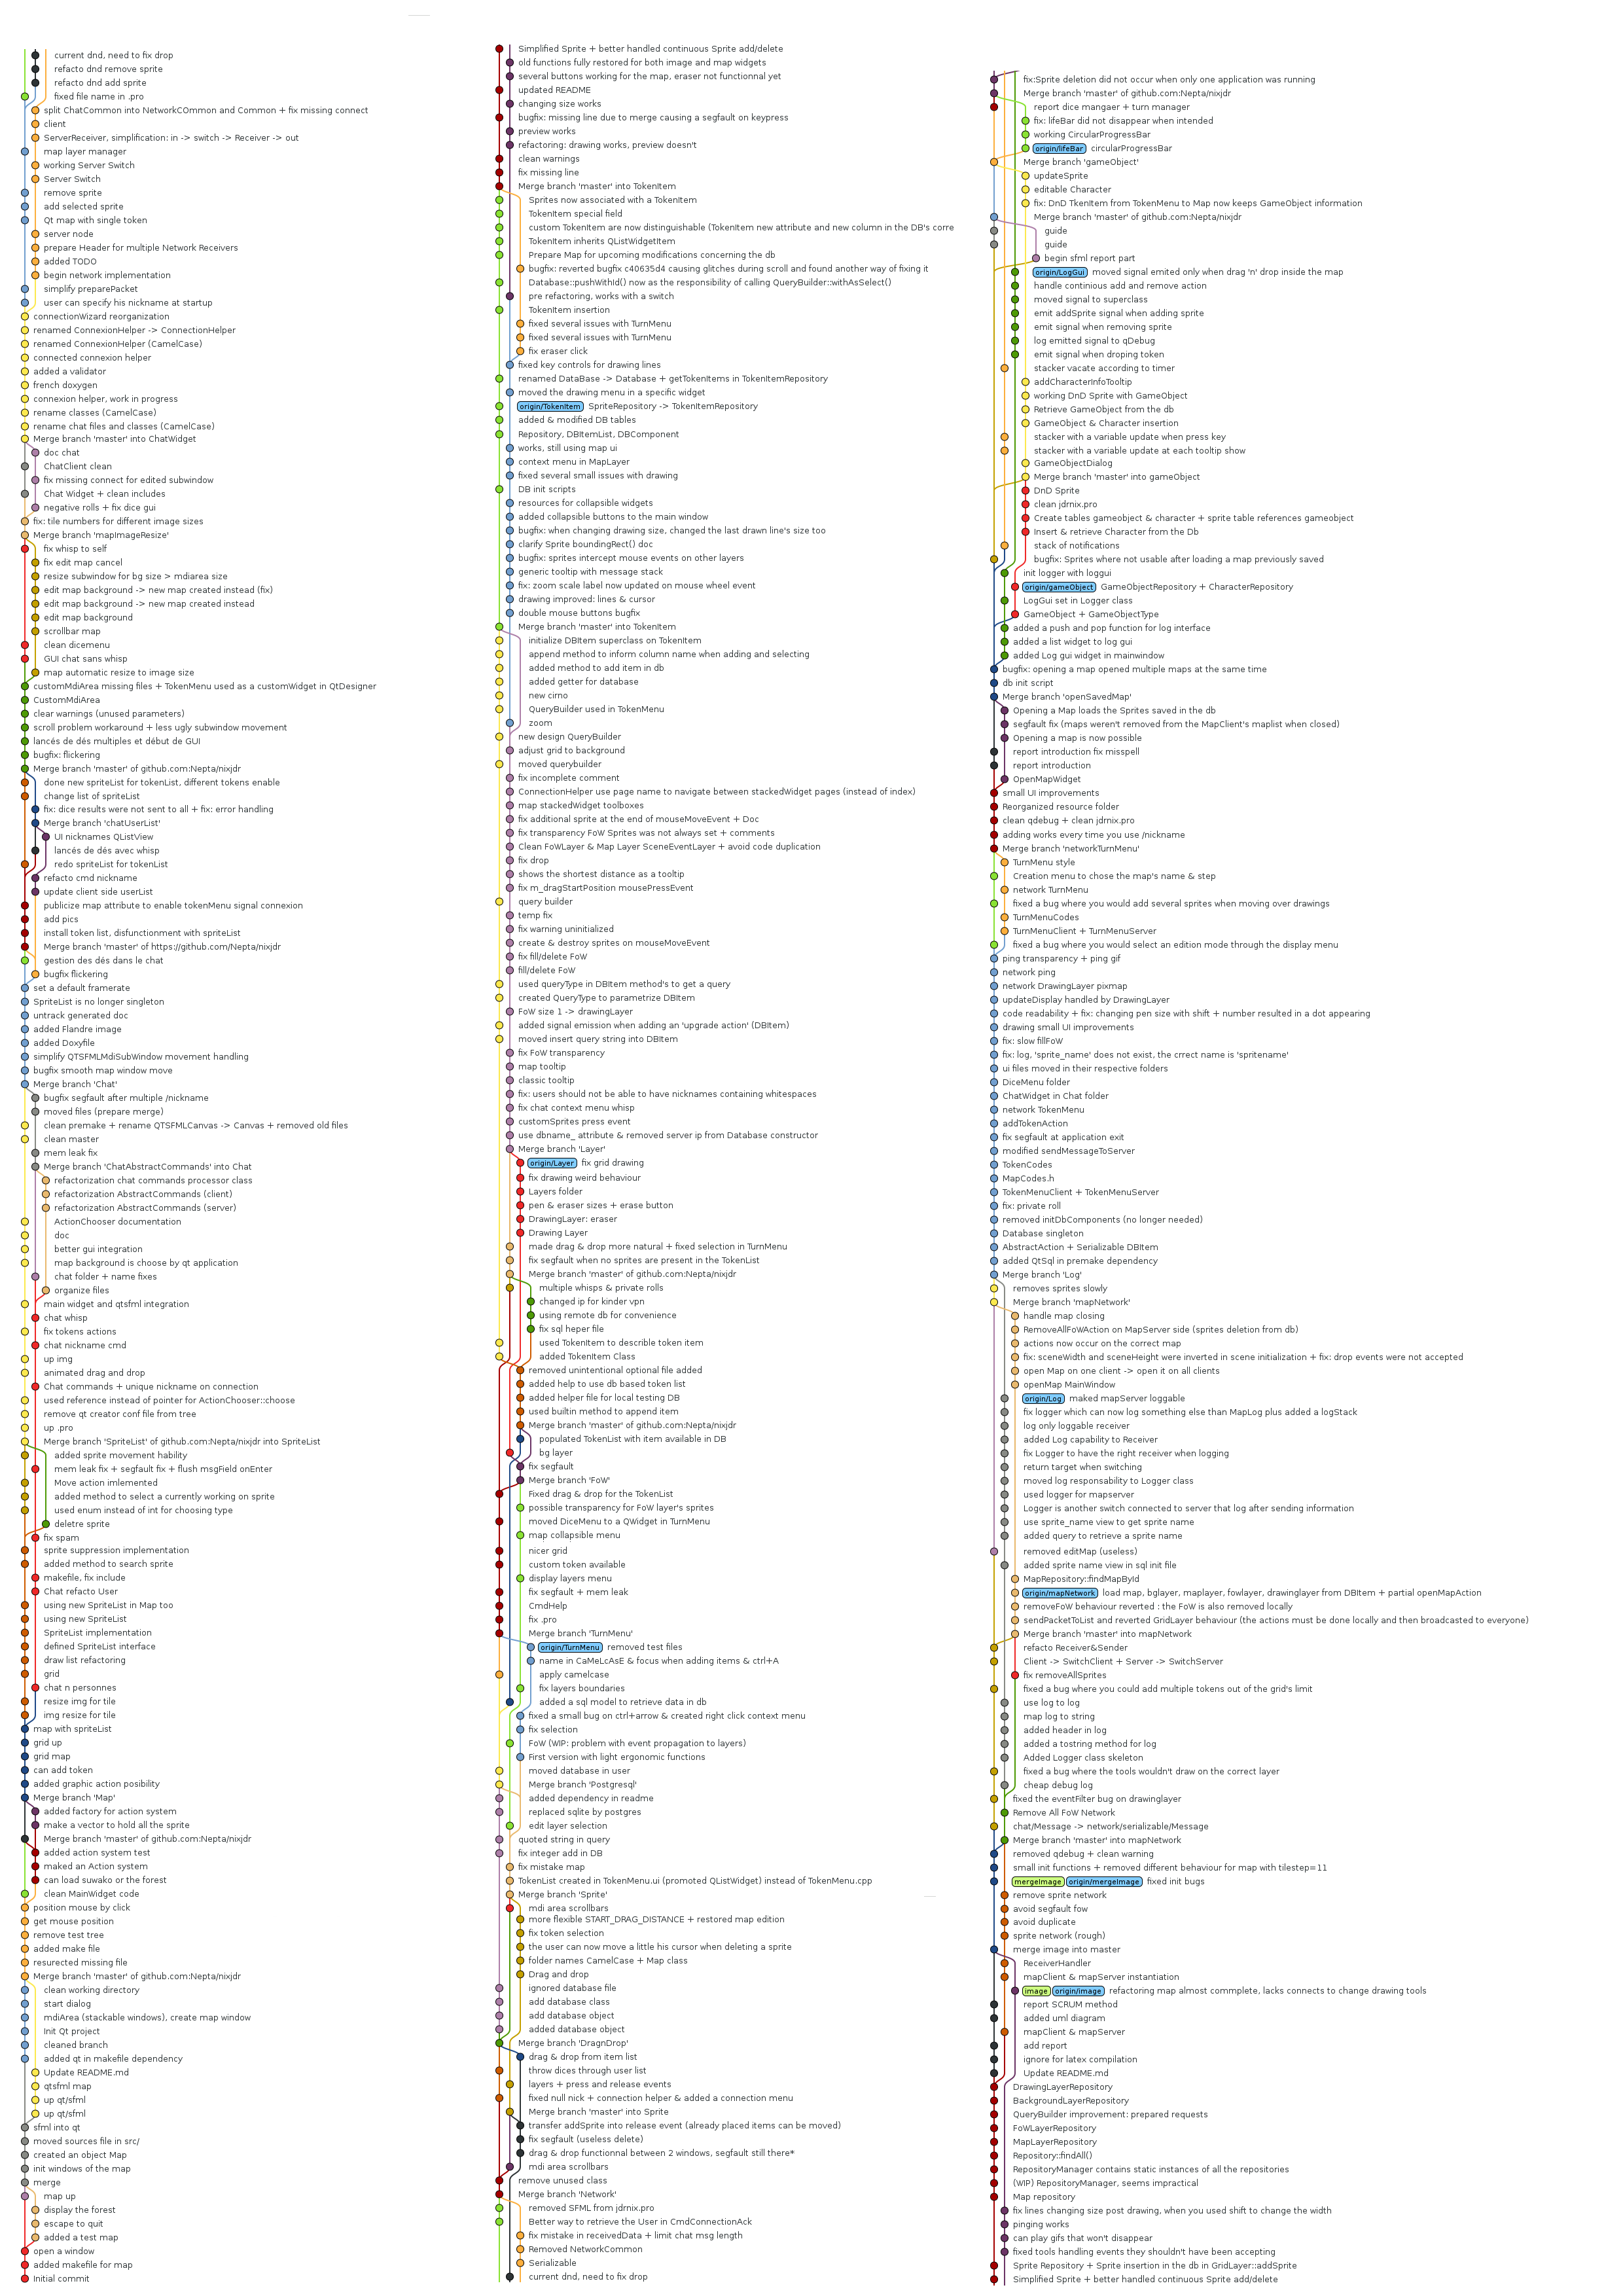
\includegraphics[width=0.5\textwidth]{img/state_git_graph.png}
	\caption{graphe des versions git}
\end{figure}

\newpage
\begin{figure}[h!]
	\centering
	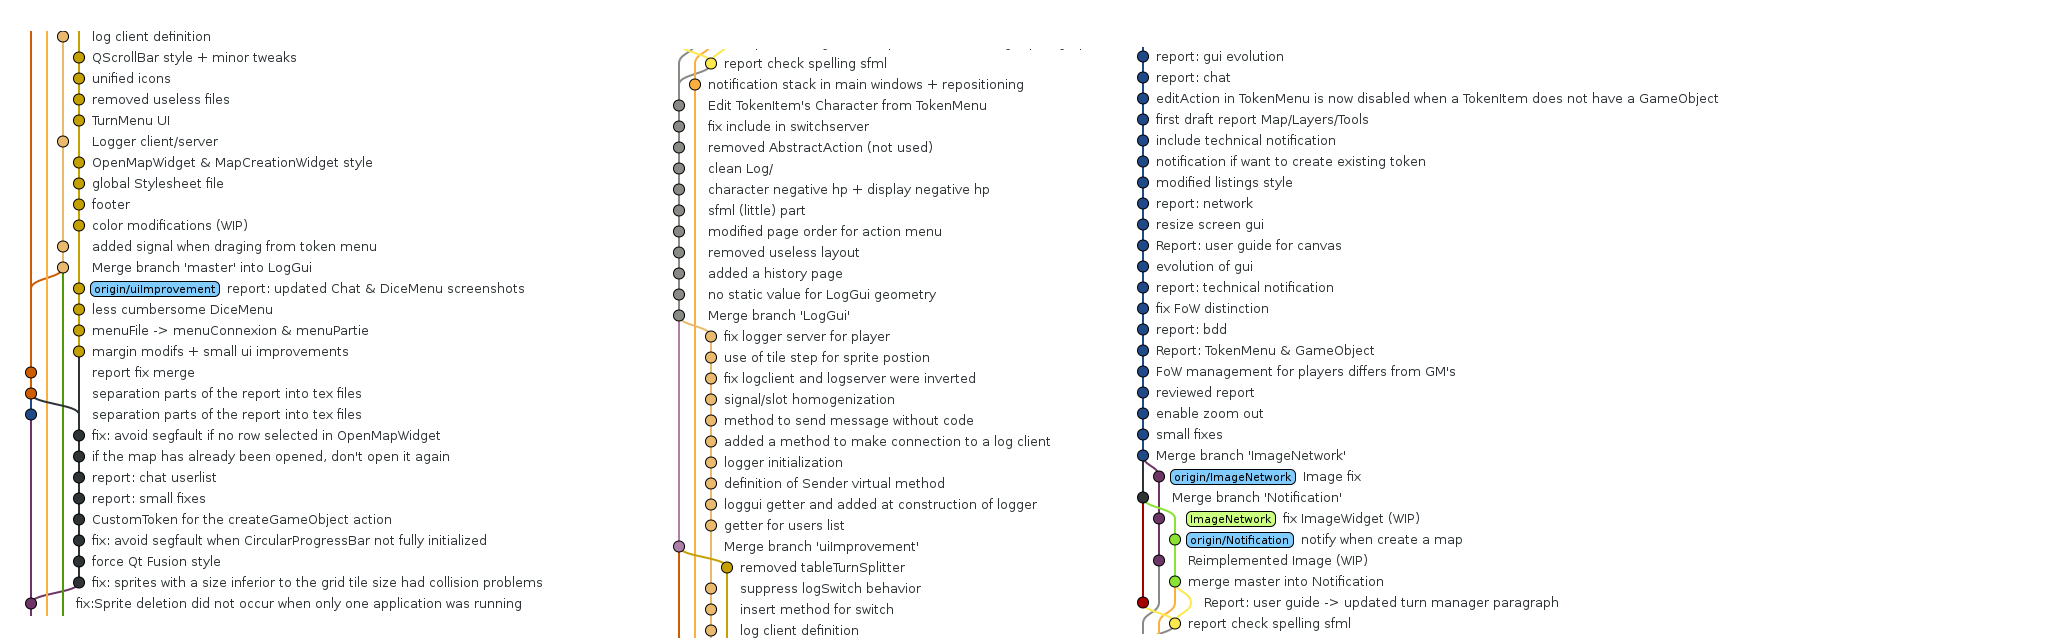
\includegraphics[width=1.0\textwidth]{img/state_git_graph_2.png}
	\caption{graphe des versions git - suite}
	\label{fig:notification}
\end{figure}
